\documentclass[english,10pt]{article}
\usepackage{babel}
%\usepackage{epigraph}
%\usepackage{quotchap}
\usepackage{csquotes}
\RequirePackage{natbib}
\RequirePackage[colorlinks,citecolor=blue,urlcolor=blue]{hyperref}
\usepackage{tikz}
\usepackage{pgfplots}
\pgfplotsset{compat=newest}
\usetikzlibrary{plotmarks}
\usetikzlibrary{arrows.meta}
\usepgfplotslibrary{patchplots}
\usepackage{graphicx}
\usepackage{subfigure}
\usepackage{setspace}
\usepackage{multirow}
\usepackage{array}
\usepackage{booktabs}
\usepackage{grffile}
\usepackage{float}
\usepackage{enumitem}
\usepackage{amsmath}
\usepackage{amsmath, amsthm, amssymb}
\usepackage{mathrsfs}
\usepackage{cleveref}
\usepackage[makeroom]{cancel}
\usepackage[section]{placeins}
\usepackage{tgbonum}
\usepackage[margin=1in]{geometry}
% \usepackage[usenames, dvipsnames]{color}
\usepackage{caption}
\usepackage{threeparttable}
\usepackage{comment}
\usepackage{subfig}
\usepackage{listings}
\usepackage{minted}
\usepackage{fontawesome5}
\usepackage{hyperref}

\makeatletter
\newcommand{\github}[1]{%
   \href{#1}{\faGithubSquare}%
}
\makeatother
\definecolor{islamicgreen}{rgb}{0.0, 0.56, 0.0}

 
%\theoremstyle{Problem}
%\newtheorem{Problem}{Problem}[section]
%\theoremstyle{Assumption}
%\newtheorem{Assumption}{Assumption}[section]
%\newtheorem{theorem}{Theorem}[section]

\usepackage{setspace}
%\doublespacing

\linespread{1.3}
%\setlength{\topmargin}{-0.3 in}
%\setlength{\mathindent}{0cm}
\title{Report: Predicting Faults in SDNs}
\author{Mohammadreza Ghobakhlou}
\date{Nov 2023}

\begin{document}

\maketitle
{\fontfamily{ppl}\selectfont}


In pursuit of enhancing network reliability and management, this research aims to establish a methodology for deriving DyNetKAT specifications from genuine Software-Defined Networking (SDN) data sets, with a focus on identifying potential malfunctions in SDN operations. The cornerstone of this approach involves the acquisition and analysis of authentic network log data, from which DyNetKAT specifications will be meticulously extracted, providing valuable insights into the underlying dynamics of these networks.

The methodology adopted in this study involves an initial phase of simulating the network to generate log files. Subsequently, these log files undergo a rigorous pre-processing phase, where their size is reduced and the network topology is extracted. The culmination of this process is the derivation of a detailed specification of DyNetKAT, which is achieved by utilizing the processed log files. This reverse engineering approach provides a novel perspective in network analysis and DyNetKAT characterization. \href{https://github.com/mghobakhlou/DyNetKAT_Spec_from_SDNLog}{\faGithubSquare \ GitHub} 


\section{Extracting Log File}

For the acquisition of log files, this study executed a systematic implementation of a firewall network, comprising one switch, two internal hosts and one external host (Figure\ref{fig:topo}), within the POX controller framework. Following this setup, a comprehensive simulation was conducted utilizing Mininet, enabling the generation and collection of pertinent log data for subsequent analysis. This approach facilitates a controlled environment for network simulation, providing valuable insights into network behavior and interactions. 


Wireshark is a widely used open-source network protocol analyzer. It allows you to capture and analyze network traffic in real-time. Wireshark supports a wide range of protocols, including OpenFlow, and provides detailed information about each packet within a network capture. Wireshark provides a graphical user interface (GUI) that displays captured packets in a readable format, allowing you to filter and search for specific network traffic.


The concurrent operation of POX, Mininet, and Wireshark enables the precise capture of OpenFlow messages exchanged between network devices and the POX controller. Utilizing Wireshark for this purpose allows for an in-depth analysis of the communication protocols and interactions within the network, thereby providing a comprehensive understanding of the network's operational dynamics. This integrated approach is instrumental in facilitating a detailed examination of network traffic and protocol behavior.

% In figure \ref{fig:wireshark_pox_log}(\href{https://drive.google.com/file/d/1JtRdAgeTsKhlbduZuVxGVlhh7Li0lHAw/view?usp=drive_link}{High quality figure}), the log extraction process involves two distinct methods for extracting log data, each showcasing different approaches. Upon examination, it becomes evident that there is no discernible distinction between these two extracted logs. Consequently, considering the inherent limitations posed by the unavailability of the controller code, the most optimal choice for log extraction is the method utilizing Wireshark. This selection aligns with the nature of the problem at hand and ensures a more effective and reliable outcome.

% \begin{figure}[h]
%     \centering
%     \includegraphics[scale = 0.2]{wireshark_pox_log.png}
%     \caption{Extracted log difference between  using controller code (left) and Wireshark (right).}
%     \label{fig:wireshark_pox_log}
% \end{figure}

\begin{figure}[t]
\centering
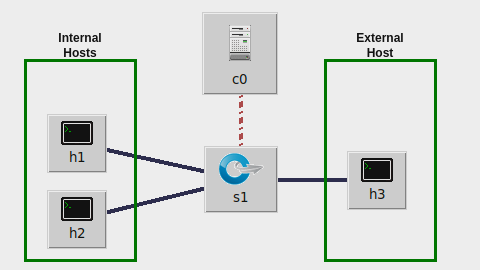
\includegraphics[scale=0.55]{topo.png}    
\caption{Network Topology}
\label{fig:topo}
\end{figure}

\section{Pre-processing}


In the current section of this study, the log files generated are subjected to a meticulous processing protocol utilizing Python and the PyShark package. This processing primarily focuses on extracting crucial data from OFPT\_FEATURES\_REPLY messages, which yields detailed insights into network topology and device-specific information. Additionally, significant information is derived from OFPT\_PACKET\_IN, OFPT\_PACKET\_OUT, and OFPT\_FLOW\_MOD messages. It is noteworthy that other message types are deemed peripheral to the objectives of this research and, as such, are not incorporated into the analysis framework.
Furthermore, as part of the data processing regimen, redundant or duplicate messages are systematically identified and eliminated to ensure the integrity and accuracy of the analysis. 


\section{Extracting DyNetKAT Terms}

The objective of this segment of the study is to ascertain the DyNetKAT specification, utilizing the data refined in the preceding phase. Employing the network topology delineated earlier, the Init policy specification is conceptualized as an ensemble of network devices policies, which are operational concurrently and in parallel. 

\[
\begin{aligned}
&Init \triangleq s1 || \ldots || sm || h1 || \ldots || hn \\
&Hosts: \{h1, \ldots, hn\}
\\
&Switches: \{s1, \ldots, sm\}
\end{aligned}\]


Each instance of detecting an OFPT\_FLOW\_MOD message signifies a modification in the switch's behavior. In this context, at the occurrence of such an event, the policy designated as si\_iteration(j) undergoes a transition, evolving into the si\_iteration(j+1) policy. This observation underscores the dynamic nature of switch operations, where policy adjustments are directly correlated with the receipt of specific network messages.


The DyNetKAT-specificication of  si\_iteration(j) are as follows.
Disjunction and conjunction between predicates are denoted by $Pr + Pr $ and $Pr . Pr$, respectively.
The policy that modifies the field $f$ of the current packet to take value $n$ is denoted by $(f \leftarrow n)$. Non-deterministic choice of DyNetKAT policies is denoted by $D\ OPLUS (\oplus)\ D$.

In the Listing \ref{json-example}, the output of the DyNetKAT description is presented, exemplifying a firewall network configuration that comprises a single switch, two internal hosts, and one external host. This example serves to demonstrate the practical application of the DyNetKAT framework in a specific network topology, offering insights into its functionality and potential use cases.



\begin{listing}
\begin{minted}[frame=single,
               framesep=3mm,
               xleftmargin=21pt,
               tabsize=8]{js}
{
    "Init": "s1_0||s1-eth1_0||s1-eth2_0||s1-eth3_0",
    "s1_0": "((openflow.eth_src: 00:00:00:00:00:00).
    (openflow.eth_dst: 00:00:00:00:00:00).
    (openflow.ofp_match.source_addr <- 0.0.0.0).
    (openflow.ofp_match.dest_addr <- 0.0.0.0).(openflow.ofp_match.source_port <- 0).
    (openflow.ofp_match.dest_port <- 0));s1_0 OPLUS CONNECTIONUP_CHANNEL?1;s1_1",
    "s1_1": "((openflow.eth_src: 00:00:00:00:00:02).
    (openflow.eth_dst: 00:00:00:00:00:01).
    (openflow.ofp_match.source_addr <- 10.0.0.2).
    (openflow.ofp_match.dest_addr <- 10.0.0.1).(openflow.ofp_match.source_port <- 0).
    (openflow.ofp_match.dest_port <- 0));s1_1 OPLUS CONNECTIONUP_CHANNEL?1;s1_2",
    "s1_2": "((openflow.eth_src: 00:00:00:00:00:01).
    (openflow.eth_dst: 00:00:00:00:00:02).
    (openflow.ofp_match.source_addr <- 10.0.0.1).
    (openflow.ofp_match.dest_addr <- 10.0.0.2).(openflow.ofp_match.source_port <- 8).
    (openflow.ofp_match.dest_port <- 0));s1_2 OPLUS CONNECTIONUP_CHANNEL?1;s1_3",
    "s1_3": "((openflow.eth_src: 00:00:00:00:00:02).
    (openflow.eth_dst: 00:00:00:00:00:01).
    (openflow.ofp_match.source_addr <- 10.0.0.2).
    (openflow.ofp_match.dest_addr <- 10.0.0.1).(openflow.ofp_match.source_port <- 0).
    (openflow.ofp_match.dest_port <- 0));s1_3 OPLUS CONNECTIONUP_CHANNEL?1;s1_4",
    "s1_4": "((openflow.eth_src: 00:00:00:00:00:02).
    (openflow.eth_dst: 00:00:00:00:00:01).
    (openflow.ofp_match.source_addr <- 10.0.0.2).
    (openflow.ofp_match.dest_addr <- 10.0.0.1).(openflow.ofp_match.source_port <- 0).
    (openflow.ofp_match.dest_port <- 0));s1_4 OPLUS CONNECTIONUP_CHANNEL?1;s1_5",
    "s1_5": "((openflow.eth_src: 00:00:00:00:00:01).
    (openflow.eth_dst: 00:00:00:00:00:02).
    (openflow.ofp_match.source_addr <- 10.0.0.1).
    (openflow.ofp_match.dest_addr <- 10.0.0.2).(openflow.ofp_match.source_port <- 0).
    (openflow.ofp_match.dest_port <- 0));s1_5 OPLUS CONNECTIONUP_CHANNEL?1;s1_6"
}
\end{minted}
\caption{DyNetKAT Specification for Firewall} 
\label{json-example}
\end{listing}




\end{document}
